%%
%% This is file `sample-sigconf.tex',
%% generated with the docstrip utility.
%%
%% The original source files were:
%%
%% samples.dtx  (with options: `sigconf')
%% 
%% IMPORTANT NOTICE:
%% 
%% For the copyright see the source file.
%% 
%% Any modified versions of this file must be renamed
%% with new filenames distinct from sample-sigconf.tex.
%% 
%% For distribution of the original source see the terms
%% for copying and modification in the file samples.dtx.
%% 
%% This generated file may be distributed as long as the
%% original source files, as listed above, are part of the
%% same distribution. (The sources need not necessarily be
%% in the same archive or directory.)
%%
%% The first command in your LaTeX source must be the \documentclass command.
\documentclass[sigplan,review]{acmart}

\usepackage{code}
\usepackage{graphicx}

%%
%% \BibTeX command to typeset BibTeX logo in the docs
\AtBeginDocument{%
  \providecommand\BibTeX{{%
    \normalfont B\kern-0.5em{\scshape i\kern-0.25em b}\kern-0.8em\TeX}}}

%% Rights management information.  This information is sent to you
%% when you complete the rights form.  These commands have SAMPLE
%% values in them; it is your responsibility as an author to replace
%% the commands and values with those provided to you when you
%% complete the rights form.
\setcopyright{acmcopyright}
\copyrightyear{2021}
\acmYear{2021}
\acmDOI{10.1145/1122445.1122456}

%% These commands are for a PROCEEDINGS abstract or paper.
\acmConference[Woodstock '18]{Woodstock '18: ACM Symposium on Neural
  Gaze Detection}{June 03--05, 2018}{Woodstock, NY}
\acmBooktitle{Woodstock '18: ACM Symposium on Neural Gaze Detection,
  June 03--05, 2018, Woodstock, NY}
\acmPrice{15.00}
\acmISBN{978-1-4503-XXXX-X/18/06}


%%
%% Submission ID.
%% Use this when submitting an article to a sponsored event. You'll
%% receive a unique submission ID from the organizers
%% of the event, and this ID should be used as the parameter to this command.
%%\acmSubmissionID{123-A56-BU3}

%%
%% The majority of ACM publications use numbered citations and
%% references.  The command \citestyle{authoryear} switches to the
%% "author year" style.
%%
%% If you are preparing content for an event
%% sponsored by ACM SIGGRAPH, you must use the "author year" style of
%% citations and references.
%% Uncommenting
%% the next command will enable that style.
%%\citestyle{acmauthoryear}

%%
%% end of the preamble, start of the body of the document source.
\begin{document}

%%
%% The "title" command has an optional parameter,
%% allowing the author to define a "short title" to be used in page headers.
\title{Let a Thousand Flowers Bloom: on the Uses of Diversity in
  Software Testing}

%%
%% The "author" command and its associated commands are used to define
%% the authors and their affiliations.
%% Of note is the shared affiliation of the first two authors, and the
%% "authornote" and "authornotemark" commands
%% used to denote shared contribution to the research.
\author{Alex Groce}
\affiliation{\institution{Northern Arizona University}\country{United States}}


%%
%% By default, the full list of authors will be used in the page
%% headers. Often, this list is too long, and will overlap
%% other information printed in the page headers. This command allows
%% the author to define a more concise list
%% of authors' names for this purpose.
\renewcommand{\shortauthors}{Alex Groce}

%%
%% The abstract is a short summary of the work to be presented in the
%% article.
\begin{abstract}
Software testing is \emph{hard}; like many real-world problems, it
offers no optimal solution, but requires dexterity, and the
opportunistic combination of many partial solutions.  Exploration and
experiment, even by practitioners, are important in real-world
critical testing efforts.  An important set of research results in the
field endorse and codify the value of \emph{diversity} in the field.
However, our current approaches to evaluating research results
arguably cut against this fundamental reality: while effective testing
may need true diversity, combining many partial answers, the iron
logic of the research results section often imposes a
\emph{totalizing} vision where authors must at least pretend to
present a monolithic Solution with a capital ``S.''
\end{abstract}

\begin{CCSXML}
<ccs2012>
<concept>
<concept_id>10011007.10010940.10010992.10010998.10011001</concept_id>
<concept_desc>Software and its engineering~Dynamic analysis</concept_desc>
<concept_significance>500</concept_significance>
</concept>
<concept>
<concept_id>10011007.10011074.10011099.10011102.10011103</concept_id>
<concept_desc>Software and its engineering~Software testing and debugging</concept_desc>
<concept_significance>500</concept_significance>
</concept>
</ccs2012>
\end{CCSXML}

\ccsdesc[500]{Software and its engineering~Dynamic analysis}
\ccsdesc[500]{Software and its engineering~Software testing and debugging}

\keywords{software testing, test diversity, swarm testing, ensemble methods,
  test length, reseach evaluation methods}


\maketitle

\section{Introduction}

Discovering all the bugs in a software system is an extremely
difficult task.  It is so difficult, in fact, that in the real world
it is seldom really attempted, for most kinds of software.  However,
when software bugs can produce catastrophic consequences, as in the
case of safety-critical software, or produce catastrophic monetary or
institutional credibility
loss (e.g., a billion dollar Mars rover mission fails because of a bug
\cite{Spirit}), it is worth at least trying to find \emph{all} the bugs,
given our difficulty in estimating the probability that an
undiscovered bug will trigger in practice.

The difficulty in discovering bugs in software is not, alas, even of
a simple kind.  It is conceivable that, while ``truly thorough testing'' or
``complete verification'' would be \emph{costly} and \emph{require
  extensive human resources}, the methods for achieving these goals
would be widely known, and omitted out of simple cost-benefit
calculations.  Unfortunately, even given willpower and budget, we
generally don't know the best way to go about trying to find all the
bugs in a system.  Complete verification, for many real-world systems,
is often essentially impossible, and even if possible would rely on a
formal specification that might not represent important requirements.
And, in testing, we seldom know which approach to testing will work
best.  Even given a particular ``method,'' such as \emph{fuzzing}, it
turns out that the ability of experts to predict which approach(es)
will be most effective is limited.  Ask ten fuzzing researchers or
practitioners what the best fuzzer is, and you won't get ten answers;
but you also probably won't get fewer than four.

Moreover, even if everyone agreed on the best fuzzer, running just
that fuzzer would likely be a bad decision!  Different fuzzers are
best at discovering different bugs, for almost all software programs.
Any competitive fuzzer that is not strictly worse than another (e.g.,
the exact same fuzzer, but slower) is likely to have some bug(s) for
which it is better than the ``best'' fuzzer.

The need for multiple approaches is even more complex when we consider
that some bugs may be best detected by code review, some bugs may be
best detected by manually written unit or integration tests, some bugs
may be best detected by turning up the toleration for false positives
in static analysis, and being willing to wade through all the
resulting complaints, and so forth.  However, even if we limit the
topic to automated test generation methods, the fact remains.  There
are a very large number of possible approaches, and users serious
about finding bugs may easily miss important bugs if they only use one
of these methods, or even if they use a few of the best methods.  In
other words, this is a situation where the utility of \emph{diversity}
is extremely high.  Diversity, here, means employing a \emph{variety} of different
methods, where in some sense many of these methods may be \emph{worse}
(on average!) than others.


This essay could, at this point, turn to marshalling evidence that a
variety of approaches, even if some are ``inferior'' to others, is
needed for finding most bugs.  The research literature and practical
commentary includes substantial evidence for this fact.  Some of it
will be cited below; however, I think this isn't really very useful.
Few software testing researchers probably don't know that there is, to
particularize Brooks' general principle \cite{Brooks1987NoSB}, ``no silver bullet'' in test
generation.  Even fewer serious practitioners of software testing who
are any good at it will think there is such a thing.  However, many
seasoned testers may use only one method, or a handful of methods,
because of the problem of diveristy.  If you are using one, known
pretty-good, method for automatically generating tests, the best
practice is likley pretty clear:  throw as many computing resources
into running this method as you can, and try to solve the hard problem
of triaging the resulting bugs and false positives you run into.  But
what if you want to use a diverse set of methods?  Learning to use one
method or tool is often time-consuming; learning to use every method
and tool sounds like a nightmare.  Two solutions offer themselves:
first, there are some ways to introduce diversity into testing even
with a single approach, that apply to many tools.  Second, there are
solutions that act as front-ends to diverse arrays of methods, saving
the bug-finder the effort of learning to ``talk'' to each approach in
its own unique language \cite{WODACommon}.

This essay will consider two aspects of this state of affairs.  First,
there is advice for the working bug-finder (developer, test engineer, systems
engineer, security auditor); what diversity-aware approaches are
available, to minimize the burden on the humble bug-finder, and make
it possible to act as if you are using one, best, method?  Second, and
perhaps in the long run 
more importantly, there is the problem that \emph{there is a serious
divergence between software testing research expectations and
publication barriers and the actual problems of software testing in a
diversity-critical world}.

\section{Digression: Diversity in General}

The idea that diversity is good is not novel, or specific to software
testing, of course.  The title of this essay is cobbled together from
famous phrases relating to the virtues of diversity \cite{chesterton,mao}.  Since, at least,
Montaigne \cite{montaigne}, Cervantes' \cite{cervantes} admonition to not ``put all your eggs in one
basket'', or perhaps the unknown Scottsman who said that it is good we all
don't like the same things, or there would be a powerful shortage of
oatmeal, diversity has been lauded, on occasion, in literature and
philosophy.  The idea of the American political system as using states
as the ``laboratory of democracy'' is essentially diversity-based, as
are arguments against too much central regulation by the European
Union.  Arguably, the same could be said for the city-states of the
ancient world (perhaps there is something to be said for both Athens
and Sparta, someone must have pointed out).  There are ethical, utilitarian, and especially,
aesthetic, arguments for preferring a multifarious rather than
monolithic, world.  This essay is only concerned with the \emph{utilitiarian}
approach to diversity exemplified by the folk saying about not putting
all your eggs in one basket.  If you only run one (very good!) fuzzer
and it happens to bad at finding the most dangerous security
vulnerability in your code, you will be at least as unhappy as the young maid
who trips and pitches her one big basket of eggs on the ground in 17th
century Spain.  We don't care (here) if diveristy is right, or
diversity is pretty, we just care that it is useful.

\section{Diversity in Practice}

In case anyone who actually goes about finding bugs in software is
reading this essay, let's start by looking at some existing ways of
making use of diversity.  The first two approaches described will
introduce ``meta-diversity'' --- diversity within a single tool or
method.  These approaches describe ways to make the behavior of a
single automated test generation method more diverse, with relatively
little effort.  They do not always apply to all methods, and, of
course, as the nature of the problem this essay faces suggests,
sometimes they don't work very well!  But they are worth trying, as
low-cost ways to add diversity when you can't, or don't want to, learn
a new method or tool.

The second approach described is fundamentally based on the uses of
diversity:  using \emph{ensemble} methods to allow a ``single'' tool
to (behind the scenes) apply many methods, with the explicity
rationale that diversity is good.

\subsection{Test Length}

Most automated test generation tools have a notion of maximum length
of the tests generated.  For fuzzers, this will often be a number of
bytes; for API-call sequence generation, it will be the number of
calls in each test.  Most tools have default values for this
parameter, and few users probably change those values.  However, the
value length can have a huge impact on the testing, and the impact is
not as simple as there being an optimal value for the length
\cite{ASE08}; different bugs may ``want'' different lengths!

\begin{figure*}
  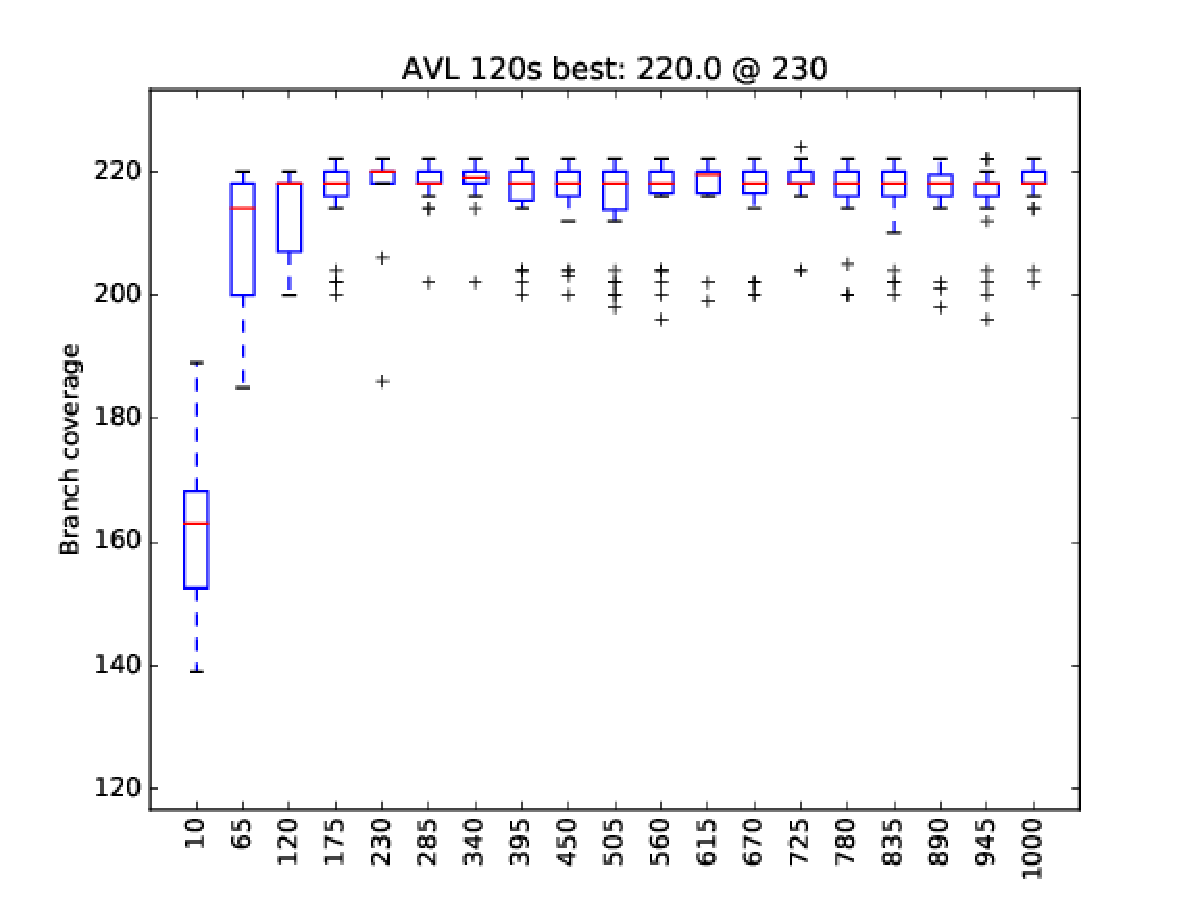
\includegraphics[width=0.9\columnwidth]{graphs/AVLrand120}
  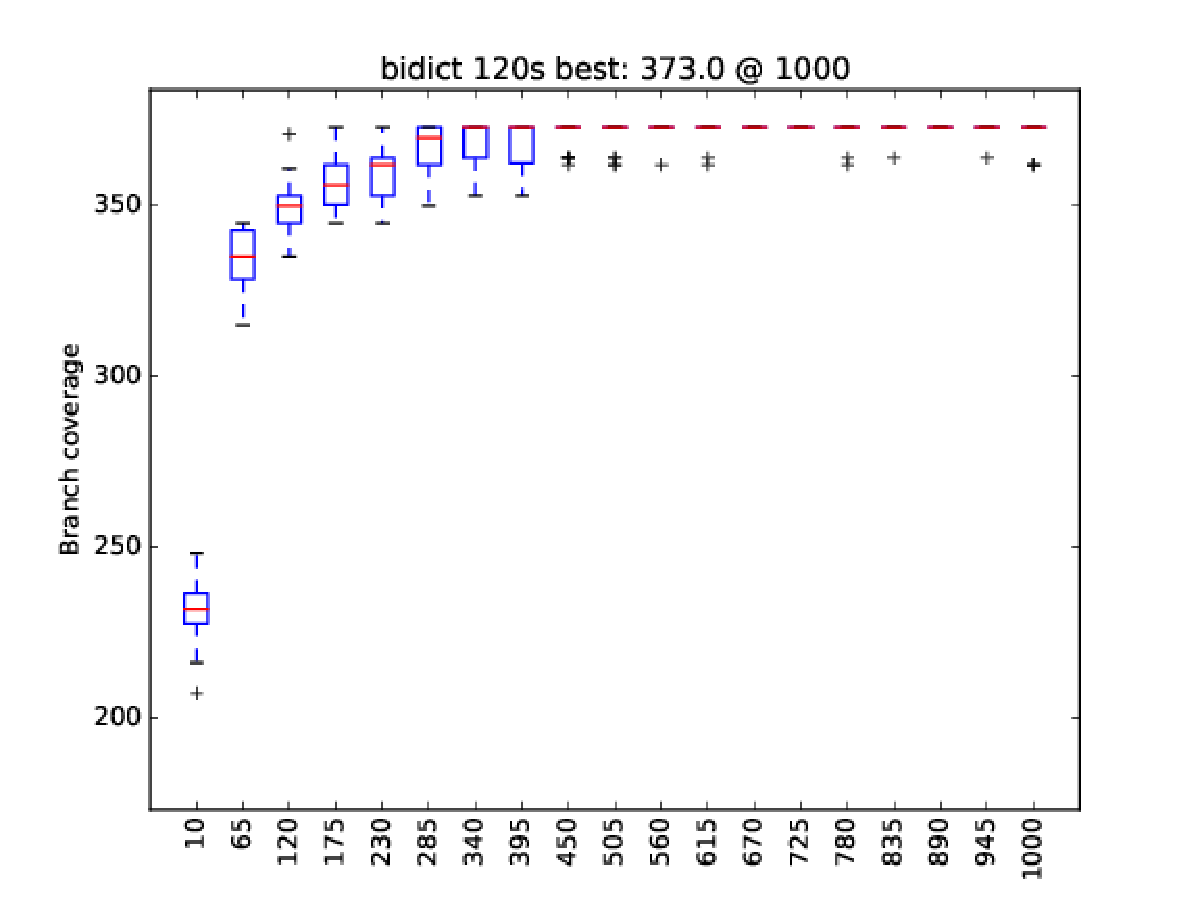
\includegraphics[width=0.9\columnwidth]{graphs/bidictrand120}
% 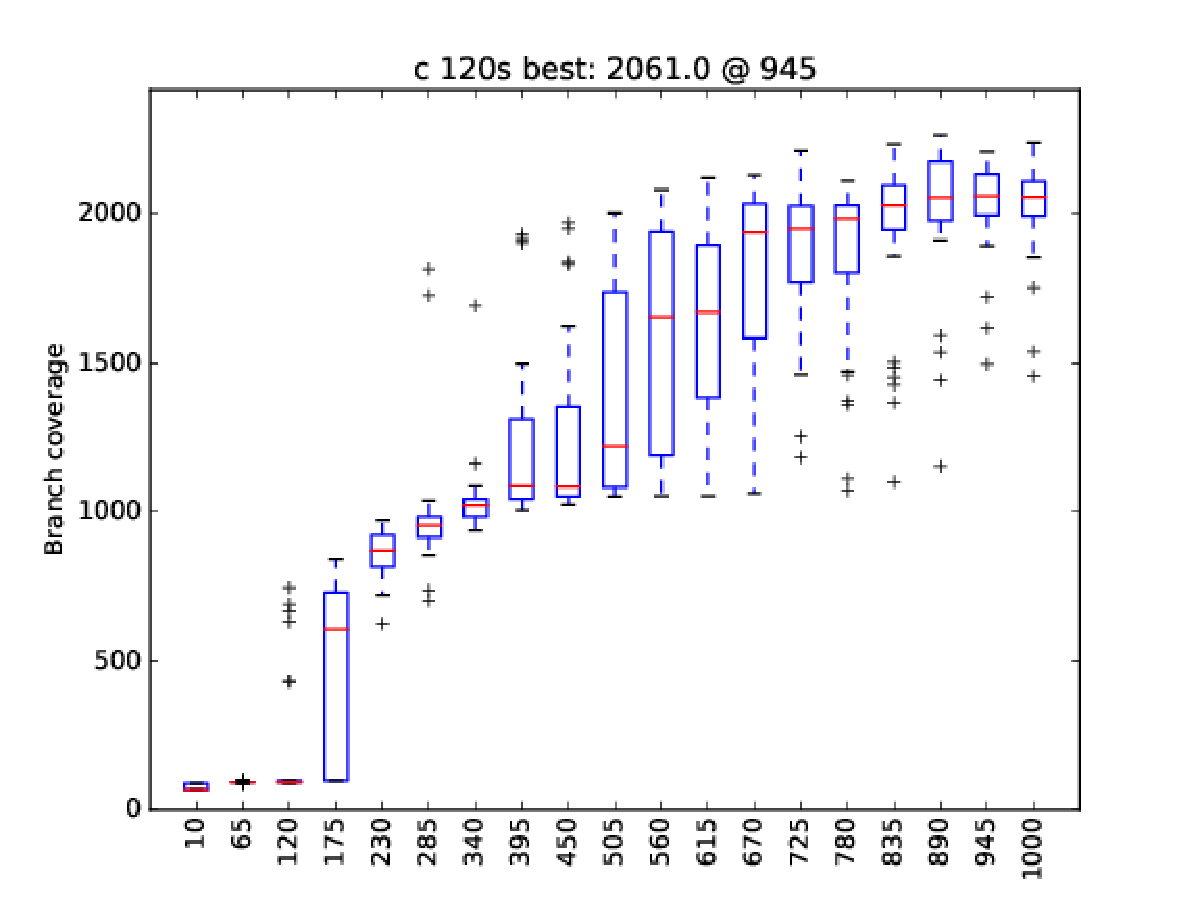
\includegraphics[width=0.9\columnwidth]{graphs/Crand120} 
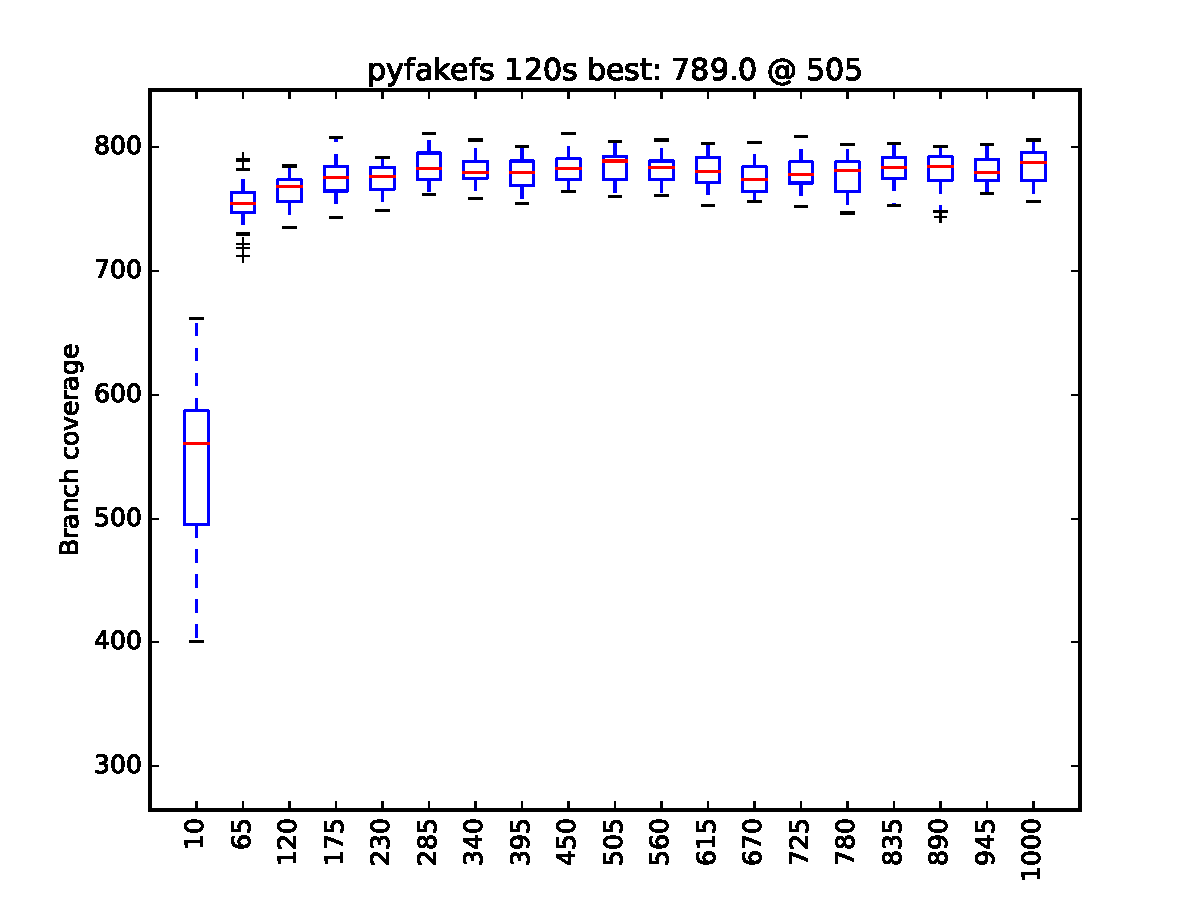
\includegraphics[width=0.9\columnwidth]{graphs/pyfakefsrand120}
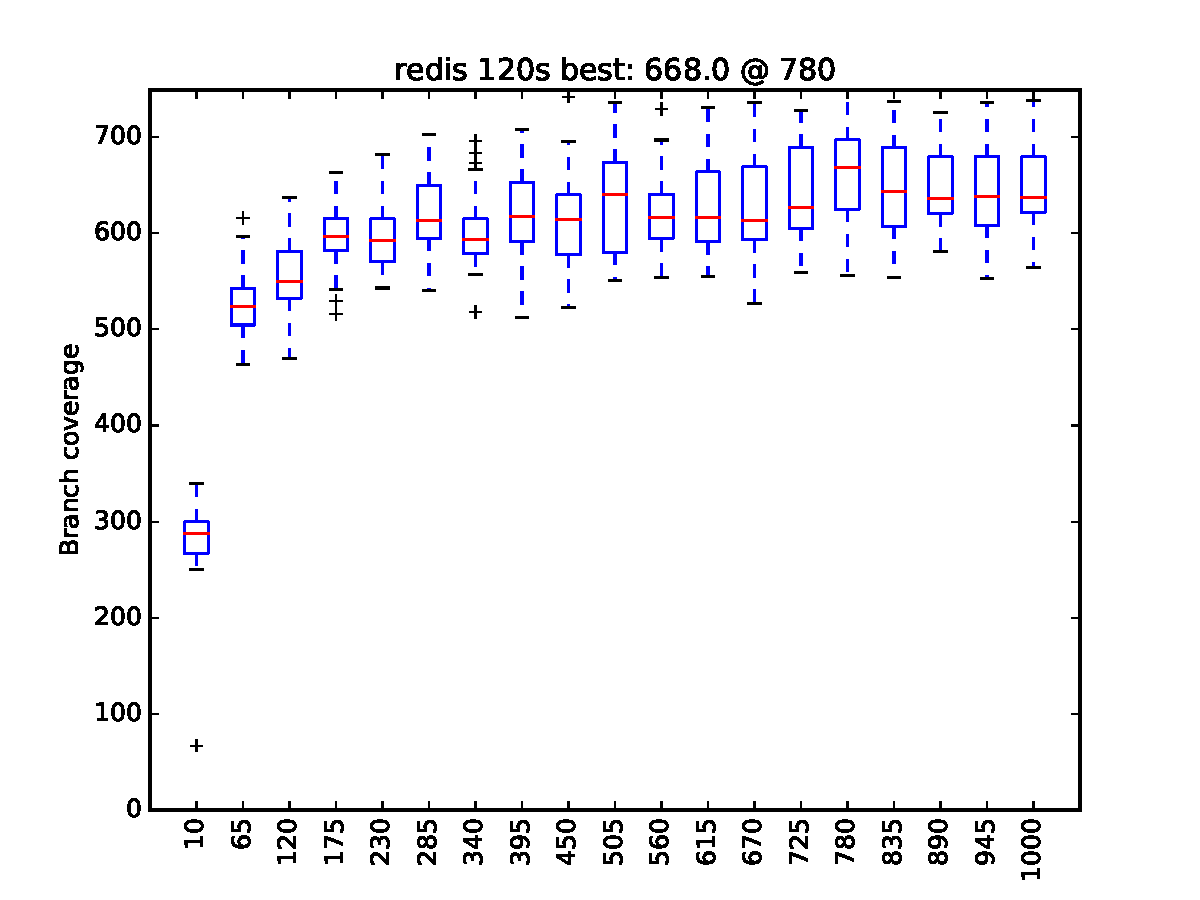
\includegraphics[width=0.9\columnwidth]{graphs/redisrand120}
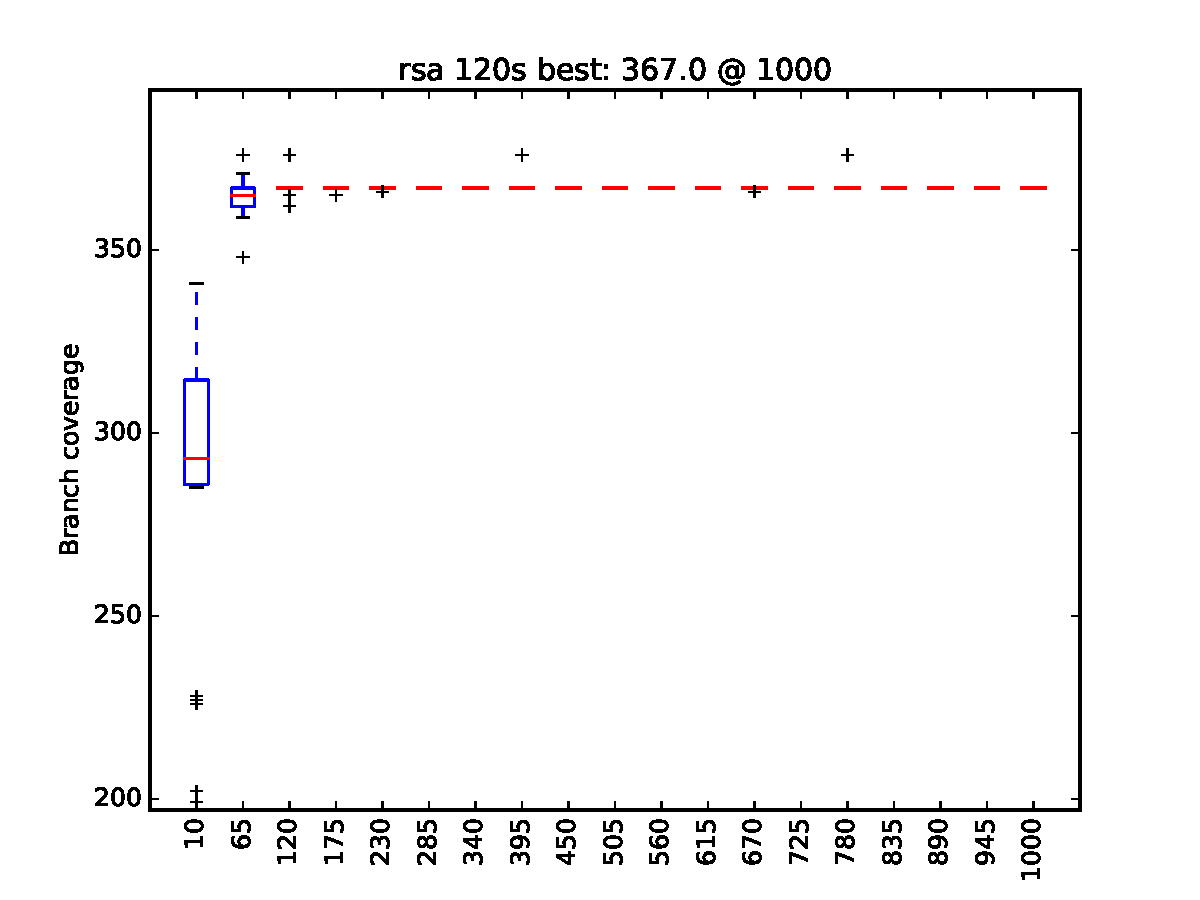
\includegraphics[width=0.9\columnwidth]{graphs/rsarand120}
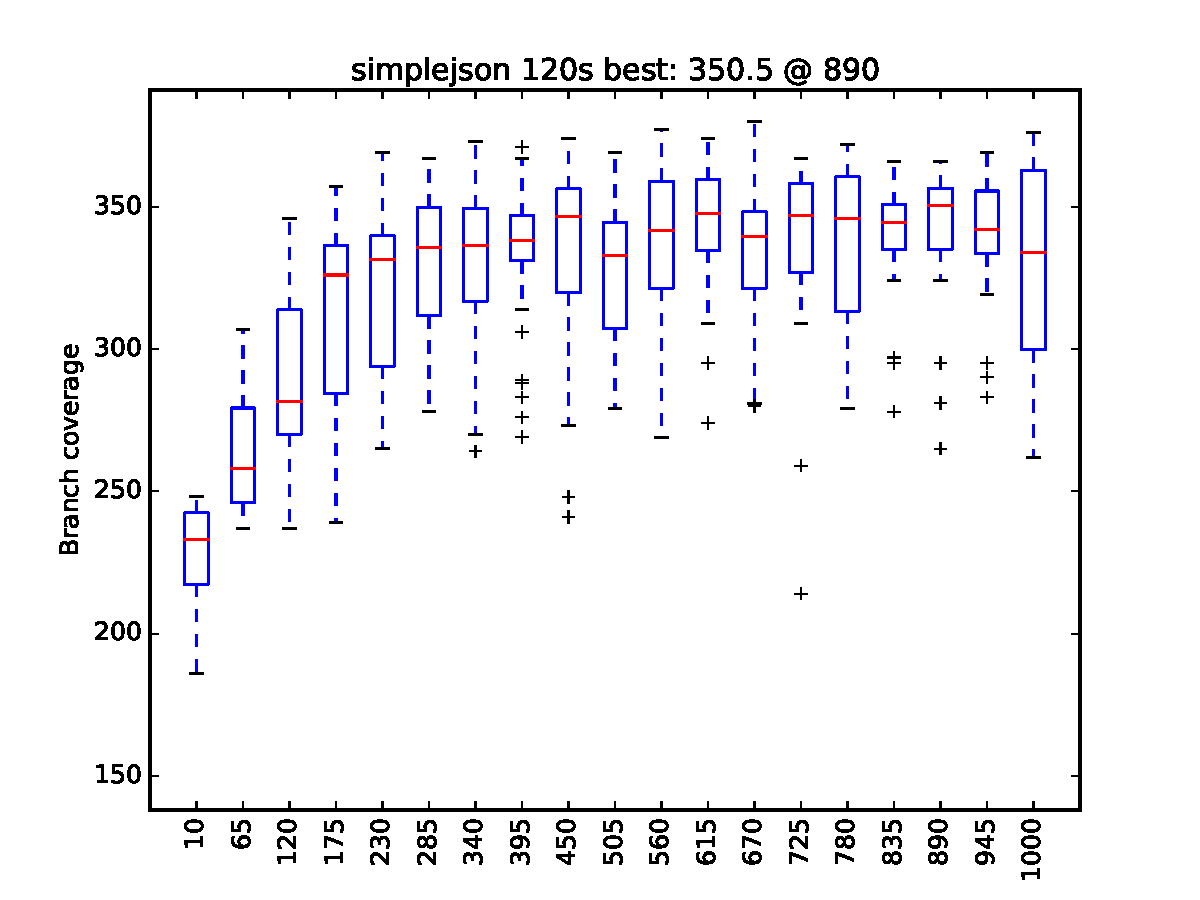
\includegraphics[width=0.9\columnwidth]{graphs/simplejsonrand120}
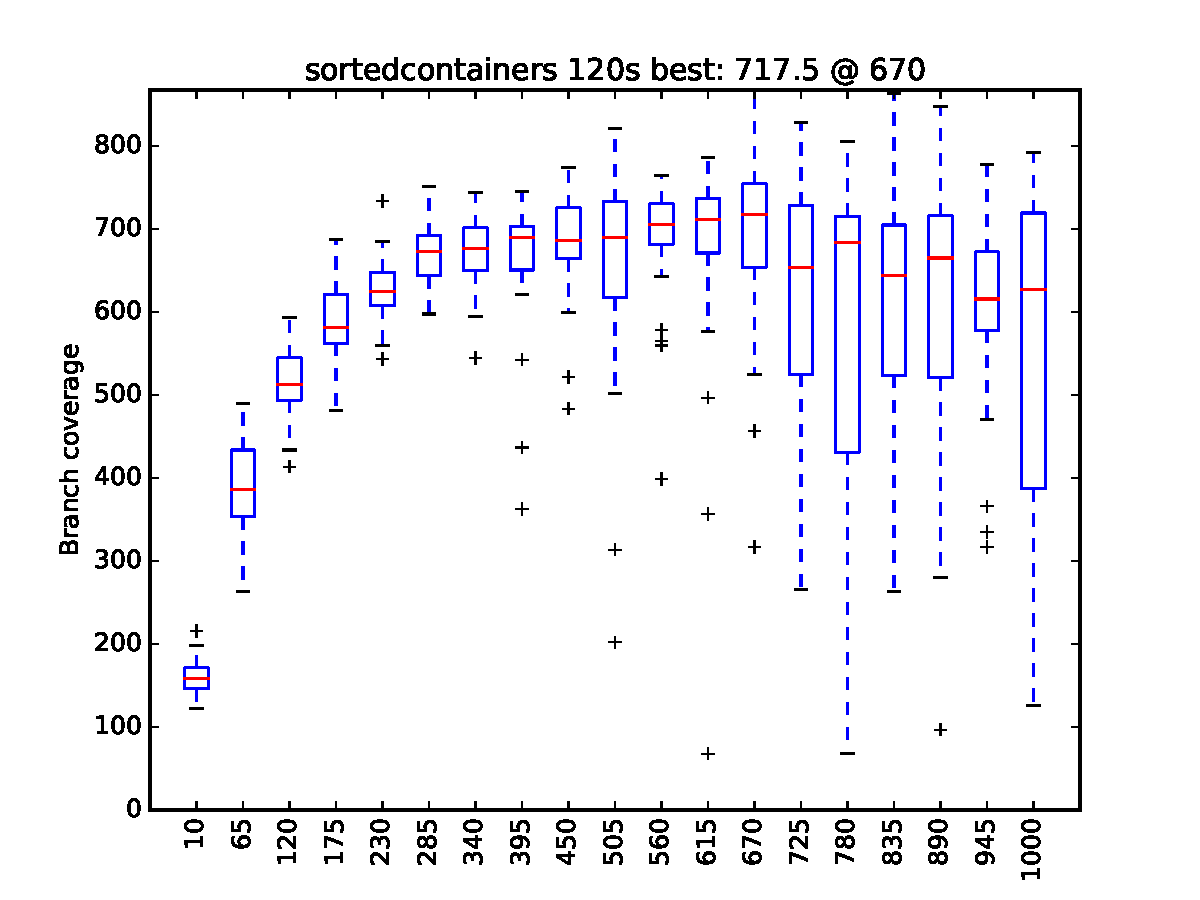
\includegraphics[width=0.9\columnwidth]{graphs/sortedcontainersrand120}
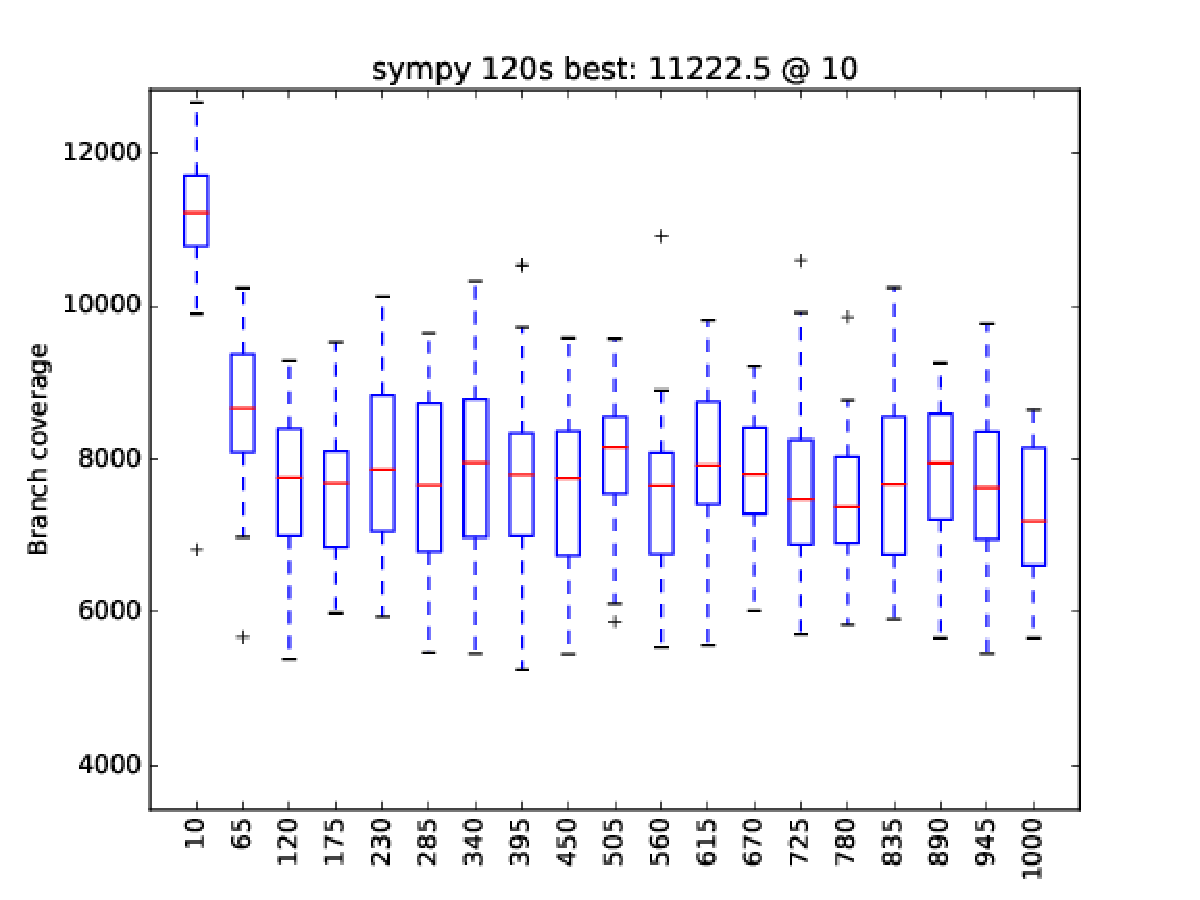
\includegraphics[width=0.9\columnwidth]{graphs/sympyrand120}
\caption{Best Test Lengths for Branch Coverage of Various Python
  Libraries}
\label{fig:length}

\end{figure*}

Figure \ref{fig:length} shows the range of branch coverage achieved in
two minute runs of the Python property-based API-sequence testing tool
TSTL \cite{tstlsttt}, for
eight real-world libraries.  The x-axis shows test sequence lengths,
and the y-axis branch coverage achieved over 100 repeated runs.  For
each method, the ``optimal'' test length is noted; this length ranges
from 10 to 1000 (the maximum length I used in experiments).  However,
just because the optimal length for a library is high or low does not
mean that some branches and bugs for that library don't need a very
different test length.  For every single target, at least two branches
were found where the optimal length for detecting \emph{that branch}
was not within 100 of the optimal value.  For {\tt pyfakefs}, {\tt
  sympy}, and {\tt sortedcontainers}, I know for a fact that real
bugs, which I reported, are most easily found using different test
length choices than the optimal value, and moreover, from each other.
In fact, for every program for which I have reported bugs, the bugs
``live'' at different test lengths.

It's not hard to understand why:  consider a bug that is caused by an
uninitialized value.  Imagine there are two function calls, {\tt foo}
and {\tt bar}.  If you call {\tt foo}, it will, as a side effect of
some other activity, initialize the uninitialized value.  In any given
test sequence, after there is a call to {\tt foo}, the bug will no
longer be detectable.  If you call {\tt bar}, but haven't first called
{\tt foo}, on the other hand, the bug will immediately be detected,
given certain choices for parameters to {\tt bar}.  In this case,
rather than running a smaller number of long tests, where any testing
after {\tt foo} is called cannot find the bug, it is best to run a
great number of fast, short, tests, in the hopes of hitting the right
{\tt bar} call before {\tt foo} shows up.

On the other hand, consider the classic overflow bug, where calling
{\tt baz} 64 times in a row causes no problems, but calling {\tt baz}
the 65th time overflows a fixed-size buffer and causes a crash.  If
there are 20 different calls that can be made, and the length of a
test is fixed at 100 calls, it's pretty hard to call {\tt baz} enough
times to trigger the bug before the ``deadline.''

As these examples show, the ``kinds of things'' that generated tests
do really vary depending on the length of tests.  In general, perhaps,
``longer is better'' \cite{ArcuriLen} but for any particular target
(bug or branch) you may be better off using diversity than optimality.

Thus, if you are using a test generation tool that lets you control
the length of inputs, and especially of call sequences, it is a very
good idea to vary the length parameter; it's a cheap way to get
significant diversity in your testing, almost like running different
tools without all the hassle!

\subsection{Swarm Techniques}

\begin{figure}
  \centering
  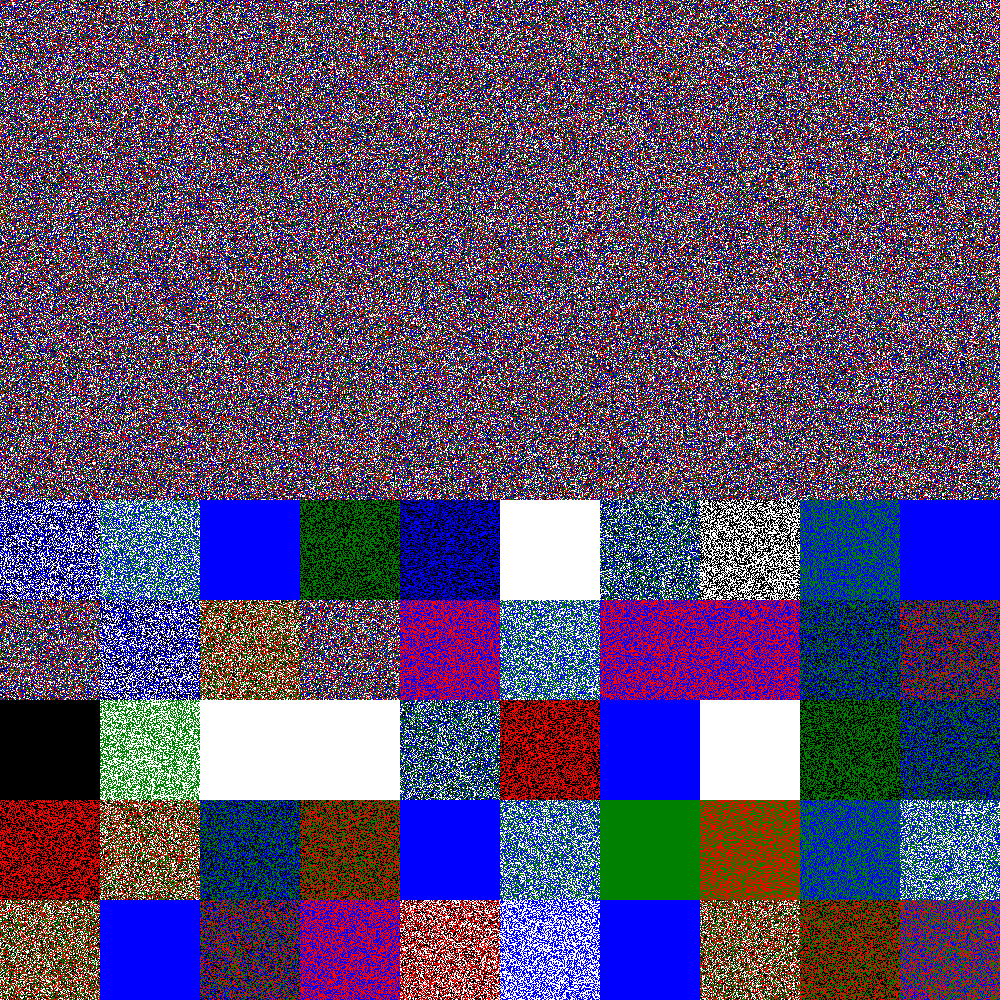
\includegraphics[width=\columnwidth]{swarm.png}
  \caption{Kitchen-sink (top) vs. Swarm (bottom)}
  \label{fig:swarmcol}
\end{figure}

Figure \ref{fig:swarmcol} shows the basic logic of swarm testing
\cite{ISSTA12}.  The figure shows a 1,000x1,000 array of pixels, where
each 10x10 block represents a sequence of 100 function calls in
an API sequence test.  Each pixel is a call to a function, and the
calls to five different functions are coded by color (black, white,
red, green, and blue).  The top half of the figure is what traditional
sequence generation will tend to do in such a setting, assuming each
call is given equal probability:  every test will look like every
other test.  The details will vary, but at a certain level the
arrangement will be very homogenous; in fact, the eye can't tell where
one test ends and another begins!  Let's call this the kitchen-sink
approach to testing:  every test generated throws in everything it can, at
least potentially.

The bottom half of the figure represents \emph{swarm testing}.  In
swarm testing, before each test is generated, a coin is flipped for
each of the five calls.  If the coin turns up ``heads'', then that
call is potentially included in the test; if the coin turns up
``tails'' the call is not made at all \emph{in this test}.  On
average, the diversity between calls within each test is \emph{much
  worse} for the swarm portion of the testing.  However, it is easy to
tell tests apart, with practical consequences.  Beyond the visually
obvious impact of swarm testing, there is simple statistical reality.
While it is \emph{possible} for a single method to be called 100 times
using the kitchen-sink approach, the most instances of any single call
we observed was 37.  For the swarm tests, of course, each method was
called more than 50 times (and in fact 100 times) in multiple tests.
The set of behaviors is simply larger, and more diverse.  You'll \emph{never}
see a pure-red, or red-green, kitchen-sink test, even if it's
technically possible.  Probability is more important than
possibility.  A million monkeys \emph{might} write Shakespeare, but
perhaps it's best not to throw away your Riverside edition, just yet.



\subsection{Ensemble Methods}

\section{The Totalizing Nature of the Experimental Results Section}


\bibliographystyle{plain}
\bibliography{bibliography}



\end{document}